\documentclass[ngerman,12pt]{scrartcl}
\usepackage[utf8x]{inputenc} 	% UTF8 für Sonderzeichen
\usepackage[a4paper,width=150mm,top=25mm,bottom=25mm]{geometry}
\linespread{1.05}				% Zeilenabstand
\usepackage{parskip} 			% Kein einrücken bei newline


\usepackage{fancyhdr}
\pagestyle{fancy}

\fancyhead{}
\fancyhead[C]{Trignometrysolver}
\fancyhead[R]{Marco Zeller}
\fancyfoot{}
\fancyfoot[C]{\thepage}

\usepackage{graphicx}
\usepackage{pgf}

%----deactivate for only compile subfiles------------
\graphicspath{{images/}}

\usepackage{amsmath,amssymb,amstext} % mathematische Symbole
\usepackage{mathtools}

% Titel
\title{Trigonometrysolver How it Works}
\author{Marco Zeller}
\date{\today}


% Formatierungen
\usepackage{shadethm}
%\usepackage[dvipsnames]{xcolor}
\usepackage{amsthm}
\usepackage{thmtools}

\declaretheoremstyle[
spaceabove=10pt, spacebelow=10pt,
headfont=\normalfont\bfseries,
notefont=\mdseries, notebraces={(}{)},
bodyfont=\normalfont,
headpunct=\\,
%postheadspace=1em,
%qed=\qedsymbol
]{mystyle}

\usepackage{cleveref}
\usepackage{nameref}

\declaretheorem[style=mystyle, name=Fall, Refname={Fall,Fälle}]{fall}
\declaretheorem[style=mystyle, name=Theorem, Refname={Theorem,Theoreme}, shaded={bgcolor=gray!15}]{theom}
\declaretheorem[style=mystyle,name=Bemerkung]{bmkg}

%Abkürzungen
\newcommand{\A}{\text{ für alle }}
\newcommand{\E}{\text{ existiert }}



\begin{document}

\maketitle

\begin{abstract}
Dieses Dokument erklärt wie der Trigonometrysolver arbeitet. Es werden aber nur die implementierten mathematischen Formeln hergeleitet, die detailierte implementation kann dem Quelltext entnommen werden.
\end{abstract}


\section{Grundlagen}

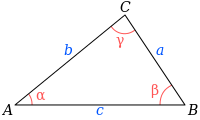
\includegraphics[scale=0.3]{Triangle_with_notations_2.png}

\begin{theom}[Innenwinkelsumme des Dreiecks]\label{sum}
Für ein beliebiges Dreieck ABC mit Winkeln $\alpha, \beta, \gamma$ gilt:

$$\pi = \alpha + \beta + \gamma$$
\end{theom}


\begin{theom}[Sinussatz]\label{sin}
Für ein belibiges Dreieck ABC mit Seiten a, b, c und Winkeln $\alpha, \beta, \gamma$ gilt:

$$ \frac{a}{\alpha} = \frac{b}{\beta} = \frac{c}{\gamma} $$
\end{theom}

\begin{theom}[Cosinussatz]\label{cos}
Für ein belibiges Dreieck ABC mit Seiten a, b, c und Winkeln $\alpha, \beta, \gamma$ gilt:

\begin{equation}
a^2 = b^2 + c^2 -2  b  c \cdot \cos(\alpha)
\end{equation}\label{cosa}
\begin{equation}
b^2 = a^2 + c^2 -2  a  c \cdot \cos(\beta)
\end{equation}\label{cosb}
\begin{equation}
c^2 = a^2 + b^2 -2  a  b \cdot \cos(\gamma)
\end{equation}\label{cosc}
\end{theom}

\section{Formeln}
\subsection{Drei Seiten bekannt}

\begin{fall}[a,b,c]\label{abc}
Aus dem \nameref{cos} folgt:
$$ \alpha =  \arccos \left(\frac{b^2 + c^2 - a^2}{2bc} \right)$$
$$ \beta =  \arccos \left( \frac{a^2 + c^2 - b^2}{2ac} \right)$$
$$ \gamma =  \arccos \left(\frac{a^2 + b^2 - c^2}{2ab} \right)$$
\end{fall}

\subsection{Drei Winkel und eine Seite}\label{wwws}
\begin{fall}[a, $\alpha,\beta,\gamma$]\label{axyz}
Aus dem \nameref{sin} folgt:
$$b = \frac{\sin(\beta)}{\sin{\alpha}} \cdot a $$
$$c = \frac{\sin(\gamma)}{\sin{\alpha}} \cdot a $$
\end{fall}
\begin{fall}[b, $\alpha,\beta,\gamma$]\label{bxyz}
Aus dem \nameref{sin} folgt:
$$a = \frac{\sin(\alpha)}{\sin{\beta}} \cdot b $$
$$c = \frac{\sin(\gamma)}{\sin{\beta}} \cdot b $$
\end{fall}
\begin{fall}[c, $\alpha,\beta,\gamma$]\label{cxyz}
Aus dem \nameref{sin} folgt:
$$a = \frac{\sin(\alpha)}{\sin{\gamma}} \cdot c $$
$$b = \frac{\sin(\beta)}{\sin{\gamma}} \cdot c $$
\end{fall}


\subsection{Zwei Winkel und eine Seite bekannt}
In diesem Abschnitt wird nicht unterschieden, welche Seite bekannt ist, da der erste Schritt des Verfahrens nicht davon abhängt und die Unterscheidung beim zweiten Schritt (Abschnitt \ref{wwws}, \Cref{axyz,bxyz,cxyz}) bereits  gemacht wurde.

\begin{fall}[$\alpha, \beta$]\label{xy}
Aus der \nameref{sum} folgt:
$$\gamma = \pi - \alpha - \beta $$
Danach wie \Cref{axyz,bxyz,cxyz}.
\end{fall}
\begin{fall}[$\alpha, \gamma$]\label{xz}
Aus der \nameref{sum} folgt:
$$\beta = \pi - \alpha - \gamma $$
Danach wie \Cref{axyz,bxyz,cxyz}.
\end{fall}
\begin{fall}[$\beta, \gamma$]\label{yz}
Aus der \nameref{sum} folgt:
$$\alpha = \pi - \beta - \gamma $$
Danach wie \Cref{axyz,bxyz,cxyz}.
\end{fall}

\subsection{Zwei Seiten und ein Winkel bekannt}
Im folgenden sind zwei Fälle zu unterscheiden:
\subsubsection{Zwei Seiten schliessen den bekannten Winkel ein}
\begin{fall}[a,b,$\gamma$]
Aus dem \nameref{cos} Formel \ref{cosc} folgt durch Wurzelziehen:
$$
c = \sqrt{a^2 + b^2 -2ab \cdot \cos(\gamma)}
$$

Danach löst man die übrigen Winkel wie im \Cref{abc} .
\end{fall}

\begin{fall}[a,c,$\beta$]
Aus dem \nameref{cos} Formel \ref{cosb} folgt durch Wurzelziehen:
$$
b = \sqrt{a^2 + c^2 -2ac \cdot \cos(\beta)}
$$

Danach löst man die übrigen Winkel wie im \Cref{abc}.
\end{fall}

\begin{fall}[b,c,$\alpha$]
Aus dem \nameref{cos} Formel \ref{cosa} folgt durch Wurzelziehen:
$$
a = \sqrt{b^2 + c^2 -2bc \cdot \cos(\alpha)}
$$

Danach löst man die übrigen Winkel wie im \Cref{abc}.
\end{fall}

\subsubsection{Winkel liegt nur an einer bekannten Seite an}
\begin{fall}[a,b,$\alpha$]
Aus dem \nameref{sin} folgt:
$$
\beta = \arcsin \left( \frac{b}{a} \sin(\alpha) \right)
$$
Danach löst man Winkel $\gamma$ wie im \Cref{xy} und Seite c wie im \Cref{axyz} oder \Cref{bxyz}.
\end{fall}

\begin{fall}[a,b,$\beta$]
Aus dem \nameref{sin} folgt:
$$
\alpha = \arcsin \left( \frac{a}{b} \sin(\beta) \right)
$$
Danach löst man Winkel $\gamma$ wie im \Cref{xy} und Seite c wie im \Cref{axyz} oder \Cref{bxyz}.
\end{fall}

\begin{fall}[a,c,$\alpha$]
Aus dem \nameref{sin} folgt:
$$
\gamma = \arcsin \left( \frac{c}{a} \sin(\alpha) \right)
$$
Danach löst man Winkel $\beta$ wie im \Cref{xz} und Seite b wie im \Cref{axyz} oder \Cref{cxyz}.
\end{fall}

\begin{fall}[a,c,$\gamma$]
Aus dem \nameref{sin} folgt:
$$
\alpha = \arcsin \left( \frac{a}{c} \sin(\gamma) \right)
$$
Danach löst man Winkel $\beta$ wie im \Cref{xz} und Seite b wie im \Cref{axyz} oder \Cref{cxyz}.
\end{fall}

\begin{fall}[b,c,$\beta$]
Aus dem \nameref{sin} folgt:
$$
\gamma = \arcsin \left( \frac{c}{b} \sin(\beta) \right)
$$
Danach löst man Winkel $\alpha$ wie im \Cref{yz} und Seite a wie im \Cref{bxyz} oder \Cref{cxyz}.
\end{fall}

\begin{fall}[b,c,$\gamma$]
Aus dem \nameref{sin} folgt:
$$
\beta = \arcsin \left( \frac{b}{c} \sin(\gamma) \right)
$$
Danach löst man Winkel $\alpha$ wie im \Cref{yz} und Seite a wie im \Cref{bxyz} oder \Cref{cxyz}.
\end{fall}



\end{document}